% Use \usepackage{graphicx}. Paths below assume compilation from the repository root.
% All results use 50 repetitions and the paper CASE mapping 11,12,13,14,15,3,16.

\begin{figure}[p]
  \centering
  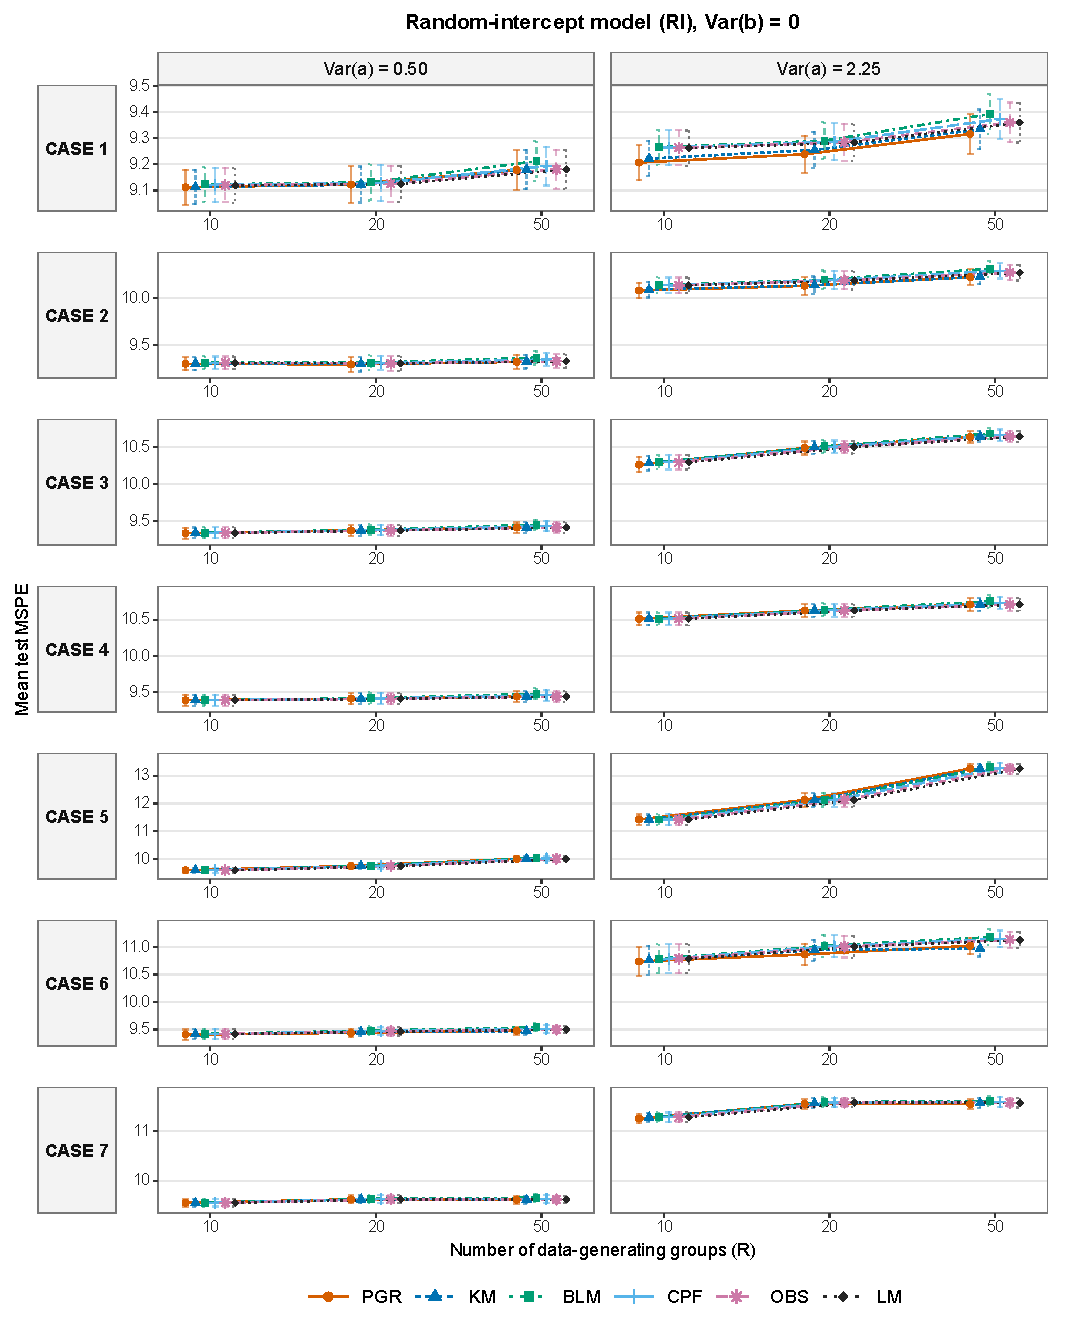
\includegraphics[width=\textwidth]{output/pdf/main_CASE1-7_RI_mean_95MC.pdf}
  \caption{Test MSPE for the random-intercept model across Cases 1--7. Columns
  correspond to $\operatorname{Var}(a)=0.50$ and $2.25$, with
  $\operatorname{Var}(b)=0$. Points are means over 50 independent repetitions;
  whiskers are approximate 95\% Monte Carlo intervals, computed as the mean
  plus or minus $1.96$ Monte Carlo standard errors. Markers are slightly offset
  horizontally for readability. The vertical scale varies by case but is shared
  across the two columns within each case.}
  \label{fig:simulation-ri}
\end{figure}

\begin{figure}[p]
  \centering
  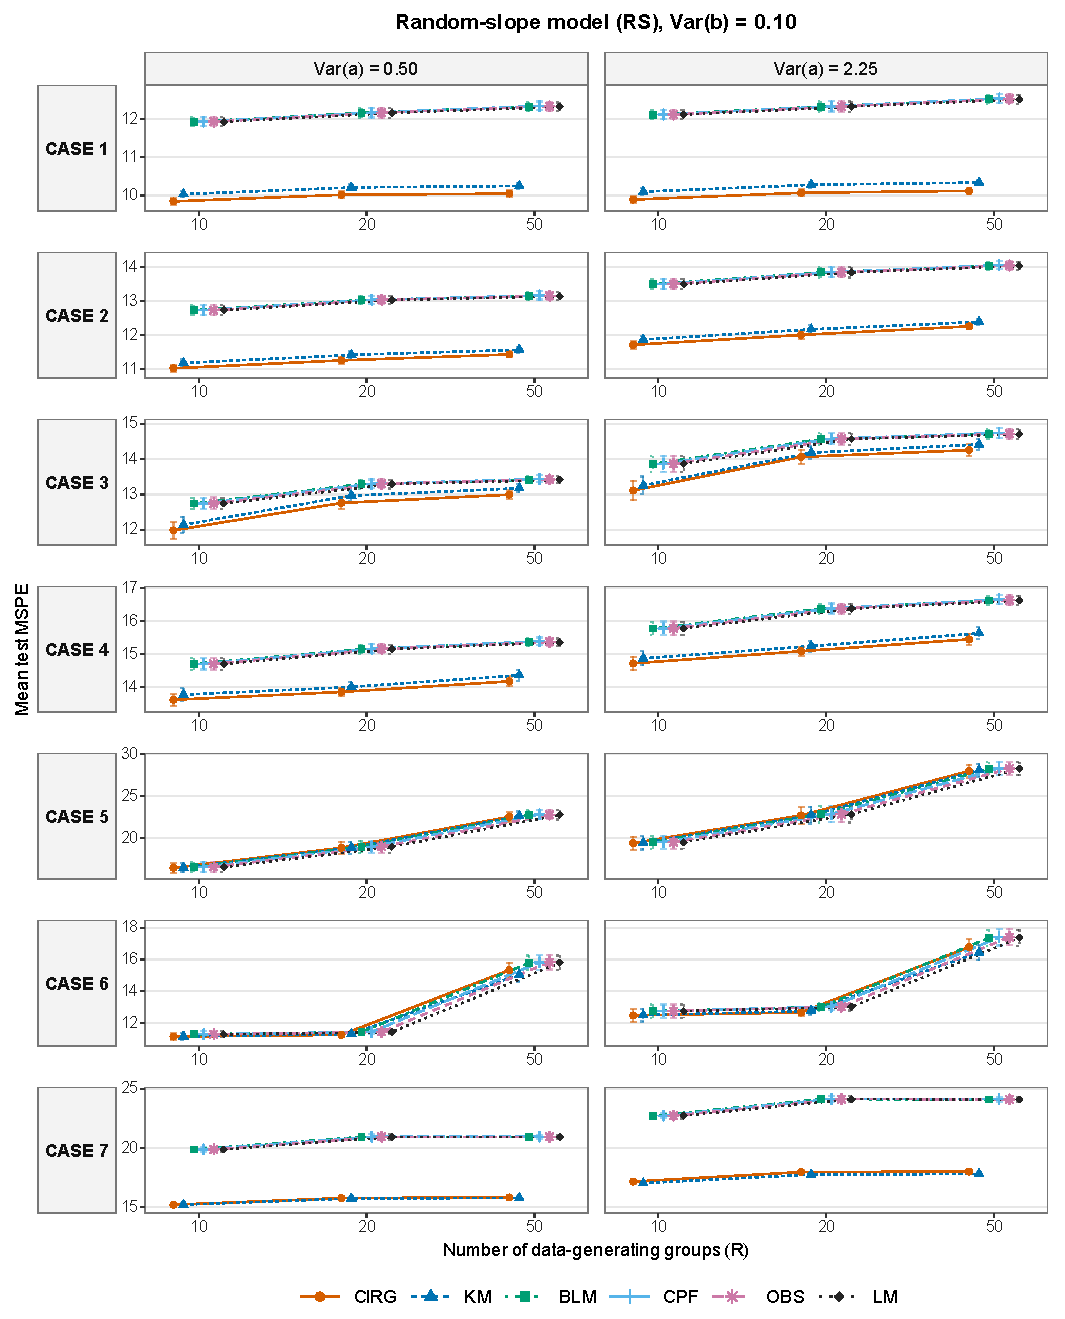
\includegraphics[width=\textwidth]{output/pdf/main_CASE1-7_RS_mean_95MC.pdf}
  \caption{Test MSPE for the random-slope model across Cases 1--7, with
  $\operatorname{Var}(b)=0.10$. Columns correspond to
  $\operatorname{Var}(a)=0.50$ and $2.25$. Points are means over 50 independent
  repetitions; whiskers are approximate 95\% Monte Carlo intervals, computed
  as the mean plus or minus $1.96$ Monte Carlo standard errors. Markers are
  slightly offset horizontally for readability. The vertical scale varies by
  case but is shared across the two columns within each case.}
  \label{fig:simulation-rs}
\end{figure}

% Include the following disclosure in the simulation protocol or figure notes:
% Finite predictions from all 50 repetitions are retained, including fits that
% reached the EM iteration limit. Convergence rates are reported separately.
% BLMX is not applicable in the absence of observed informative individual
% moments and is therefore omitted. CPF and BLM are the operational adaptations
% specified in the simulation protocol. The residual weight is fixed at zero.

% Alternative to the two combined figures: one figure per paper CASE.
\newcommand{\simulationcasefigure}[2]{%
  \begin{figure}[t]
    \centering
    \includegraphics[width=\textwidth]{output/pdf/CASE#2_mean_95MC.pdf}
    \caption{Simulation result for CASE#1. Top: random-intercept model,
    $\operatorname{Var}(b)=0$; bottom: random-slope model,
    $\operatorname{Var}(b)=0.10$. Columns correspond to
    $\operatorname{Var}(a)=0.50$ and $2.25$. Points show mean test MSPE over
    50 independent repetitions; whiskers are approximate 95\% Monte Carlo
    intervals (mean $\pm 1.96$ Monte Carlo standard errors). Panel-specific
    vertical scales are used. Markers are slightly offset horizontally.}
    \label{fig:case#1}
  \end{figure}%
}
\simulationcasefigure{1}{01}
\simulationcasefigure{2}{02}
\simulationcasefigure{3}{03}
\simulationcasefigure{4}{04}
\simulationcasefigure{5}{05}
\simulationcasefigure{6}{06}
\simulationcasefigure{7}{07}

% Supplementary robustness figures. Repeat with RS for the random-slope model.
\begin{figure}[p]
  \centering
  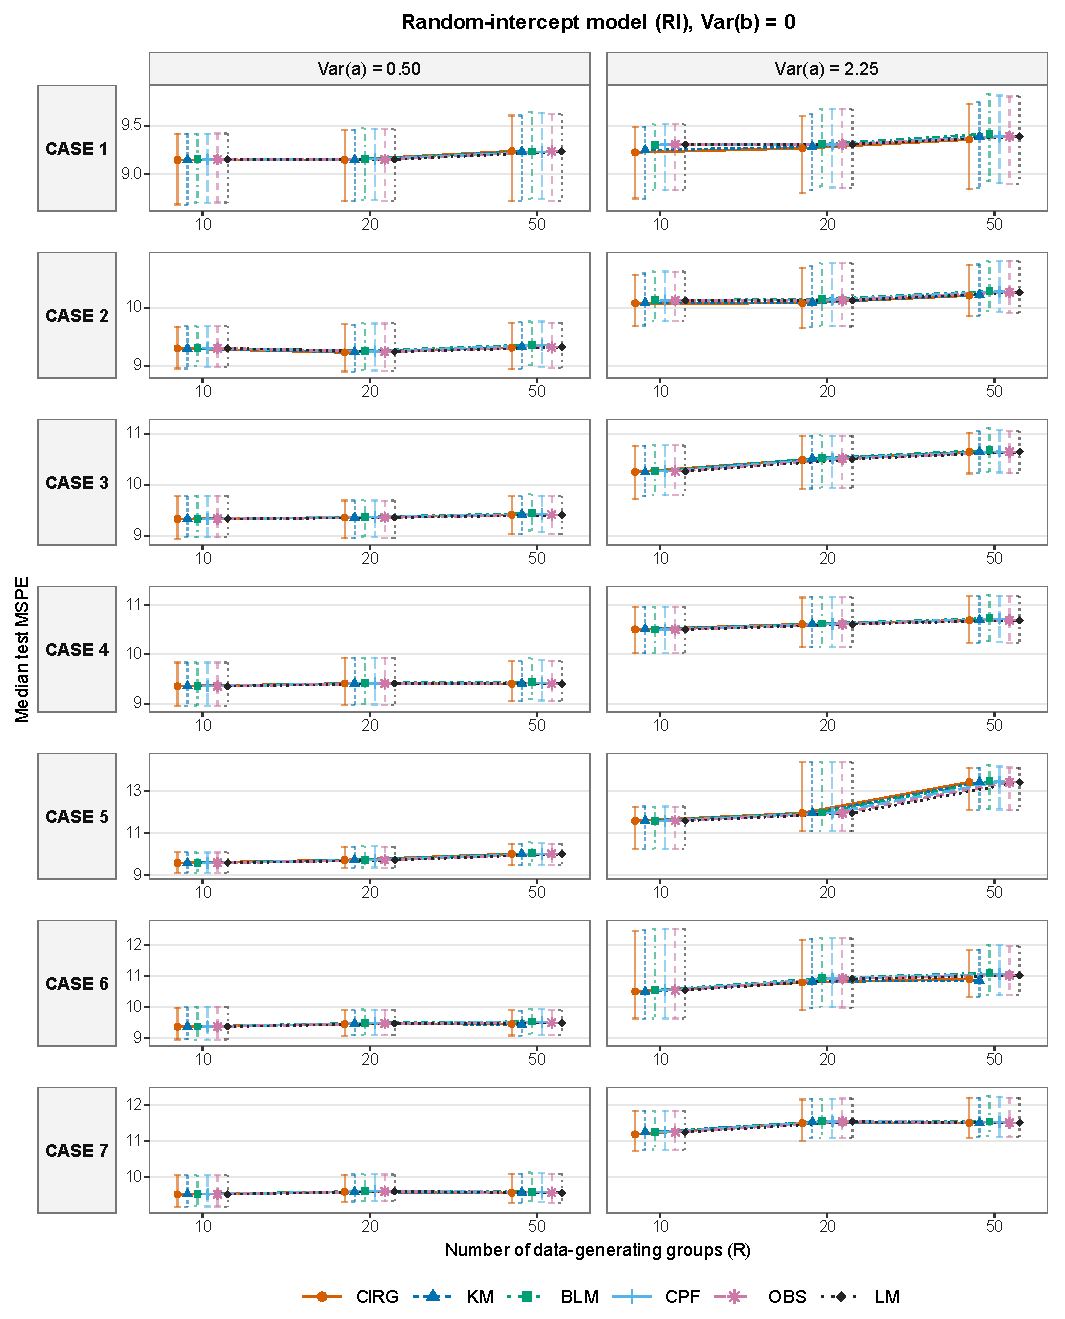
\includegraphics[width=\textwidth]{output/pdf/robustness_CASE1-7_RI_median_Q05-Q95.pdf}
  \caption{Between-repetition variability in test MSPE for the random-intercept
  model. Points show medians across 50 repetitions; whiskers span the empirical
  5th--95th percentiles (R quantile type 7). These are descriptive spread
  intervals, not confidence intervals for the mean or prediction intervals
  for individual responses. Markers are slightly offset horizontally.}
  \label{fig:robustness-ri}
\end{figure}
